\begin{example}\label{example:matching}
    Consider the following example with \(S = \{A, B, C\}\) and \(R = \{D, E,
    F\}\). We can visualise this matching game as a bipartite graph as in
    Figure~\ref{fig:matching_bipartite}. In this representation, an edge between
    two vertices indicates that they are matched by \(M\). Beside each node is 
    the name of the node and a complete ranking of its complementary set's 
    elements. We interpret these rankings as the values of our preference list 
    functions. Here, for instance, \(A\) would most prefer to be matched with 
    \(D\), then \(E\), and finally \(F\).
    
    \begin{figure}[h]
        \centering
        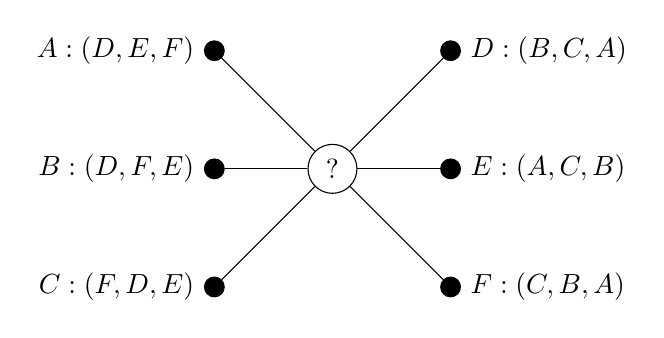
\begin{tikzpicture}[scale=0.5]

    % Suitors
    \node[draw, shape=circle, fill, inner sep=0, minimum size=0.25cm,
    label=left: {\(A: (D, E, F)\)}] (A) at (0, 0) {};
    \node[draw, shape=circle, fill, inner sep=0, minimum size=0.25cm, 
    label=left: {\(B: (D, F, E)\)}] (B) at (0, -3) {}; 
    \node[draw, shape=circle, fill, inner sep=0, minimum size=0.25cm, 
    label=left: {\(C: (F, D, E)\)}] (C) at (0, -6) {};

    % Reviewers
    \node[draw, shape=circle, fill, inner sep=0, minimum size=0.25cm, 
    label=right: {\(D: (B, C, A)\)}] (D) at (6, 0) {};
    \node[draw, shape=circle, fill, inner sep=0, minimum size=0.25cm, 
    label=right: {\(E: (A, C, B)\)}] (E) at (6, -3) {};
    \node[draw, shape=circle, fill, inner sep=0, minimum size=0.25cm,
    label=right: {\(F: (C, B, A)\)}] (F) at (6, -6) {};

    % Question mark node
    \node[draw, shape=circle] (q) at (3, -3) {?};
        
    % Lines into (?)
    \foreach \x in {A, B, C, D, E, F}
        \draw (\x) -- (q);

\end{tikzpicture}
\caption{A simple matching game represented on a bipartite
    graph.}\label{fig:matching_bipartite}

    \end{figure}

    Suppose we have the matching shown in Figure~\ref{fig:unstable_matching} for
    our game. This matching, \(M\) is valid since it is a bijection between 
    \(S\) and \(R\) but it is not stable. For instance, we have \((B, D)\) as a
    blocking pair since \(B\) would rather be matched with \(D\) than its 
    current match \(E\), and \(D\) would prefer to be matched with \(B\) than
    its current match \(A\).

    \begin{figure}[h]
        \centering
        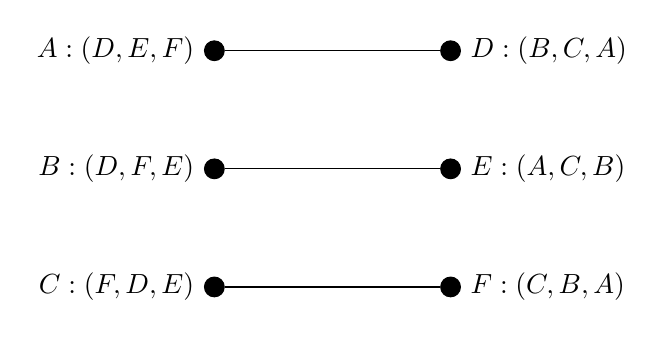
\begin{tikzpicture}[scale=0.5]

    % Suitors
    \node[draw, shape=circle, fill, inner sep=0, minimum size=0.25cm, 
    label=left: {\(A: (D, E, F)\)}] (A) at (0, 0) {};
    \node[draw, shape=circle, fill, inner sep=0, minimum size=0.25cm, 
    label=left: {\(B: (D, F, E)\)}] (B) at (0, -3) {}; 
    \node[draw, shape=circle, fill, inner sep=0, minimum size=0.25cm, 
    label=left: {\(C: (F, D, E)\)}] (C) at (0, -6) {};

    % Reviewers
    \node[draw, shape=circle, fill, inner sep=0, minimum size=0.25cm, 
    label=right: {\(D: (B, C, A)\)}] (D) at (6, 0) {};
    \node[draw, shape=circle, fill, inner sep=0, minimum size=0.25cm, 
    label=right: {\(E: (A, C, B)\)}] (E) at (6, -3) {};
    \node[draw, shape=circle, fill, inner sep=0, minimum size=0.25cm,
    label=right: {\(F: (C, B, A)\)}] (F) at (6, -6) {};

    % Lines
    \draw (A) -- (D);
    \draw (B) -- (E);
    \draw (C) -- (F);

\end{tikzpicture}
\caption{A example of an unstable matching for our
    game.}\label{fig:unstable_matching}

    \end{figure}

    We can make this matching stable by switching these pairs as in
    Figure~\ref{fig:stable_matching}. Here we have that each suitor is matched 
    with their most preferred reviewer so as not to form a blocking pair. We 
    call such a matching \emph{suitor-optimal}.

    \begin{figure}[h]
        \centering
        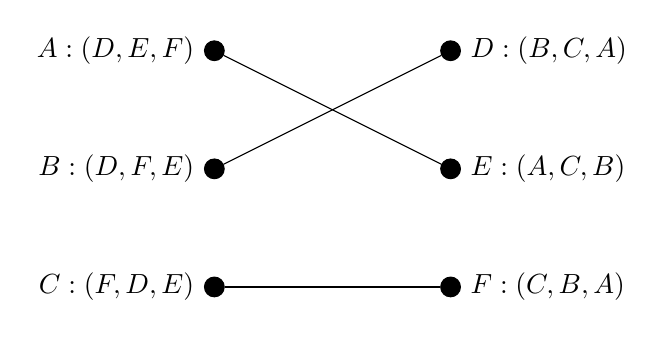
\begin{tikzpicture}[scale=0.5]

    % Suitors
    \node[draw, shape=circle, fill, inner sep=0, minimum size=0.25cm, 
    label=left: {\(A: (D, E, F)\)}] (A) at (0, 0) {};
    \node[draw, shape=circle, fill, inner sep=0, minimum size=0.25cm, 
    label=left: {\(B: (D, F, E)\)}] (B) at (0, -3) {}; 
    \node[draw, shape=circle, fill, inner sep=0, minimum size=0.25cm, 
    label=left: {\(C: (F, D, E)\)}] (C) at (0, -6) {};

    % Reviewers
    \node[draw, shape=circle, fill, inner sep=0, minimum size=0.25cm, 
    label=right: {\(D: (B, C, A)\)}] (D) at (6, 0) {};
    \node[draw, shape=circle, fill, inner sep=0, minimum size=0.25cm, 
    label=right: {\(E: (A, C, B)\)}] (E) at (6, -3) {};
    \node[draw, shape=circle, fill, inner sep=0, minimum size=0.25cm,
    label=right: {\(F: (C, B, A)\)}] (F) at (6, -6) {};

    % Lines
    \draw (A) -- (E);
    \draw (B) -- (D);
    \draw (C) -- (F);

\end{tikzpicture}
\caption{An example of a stable matching for our
    game.}\label{fig:stable_matching}

    \end{figure}
\end{example}
